Foram selecionados os tópicos mais relevantes para o contexto do presente trabalho quanto aos planos de gerenciamento propostos pelo PMBOK. Serão abordados tópicos a cerca dos planos de gerenciamento de escopo, aquisições, recursos humanos, riscos  e tempo.

\section{Escopo}

\subsection{Estrutura Analítica do Projeto e do Produto}

Para comunicar os entregáveis que compõem o produto, foi ilustrada a EAP do produto conforme a Figura \ref{fig:eap_produto}.

\begin{figure}[htpb!]
    \centering
    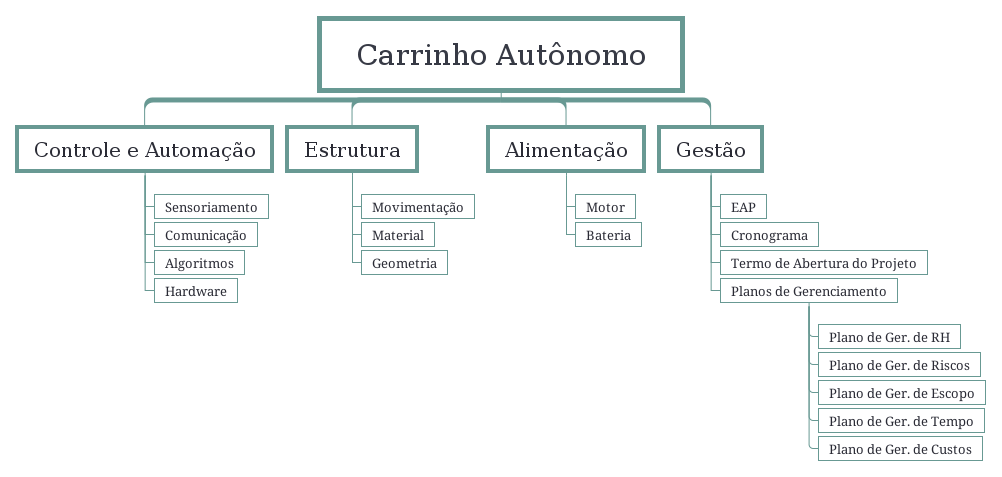
\includegraphics[scale= 0.4]{figuras/eap_produto.png}
    \caption{EAP do Produto. Fonte: Autores.}
    \label{fig:eap_produto}
\end{figure}

Para comunicar os entregáveis que compõem o projeto, foi ilustrada a EAP do projeto conforme a Figura \ref{fig:eap_projeto}.

\begin{figure}[htpb!]
    \centering
    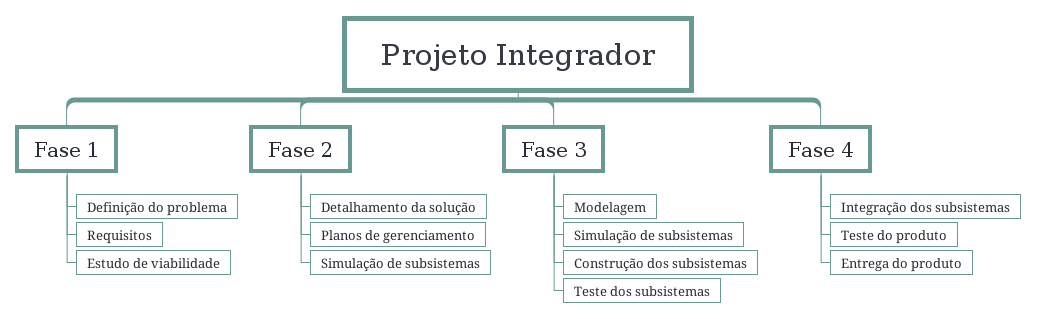
\includegraphics[scale= 0.35]{figuras/eap_projeto.png}
    \caption{EAP do Projeto. Fonte: Autores.}
    \label{fig:eap_projeto}
\end{figure}

\pagebreak

\section{Recursos humanos}

\subsection{Responsabilidades}
Os recursos humanos que foram mobilizados para este projeto e suas responsabilidades são detalhados na Tabela \ref{tab:responsabilidades}.


% ######## init table ########
\begin{table}[h]
\caption {Detalhamento das responsabilidades} \label{tab:responsabilidades} 
 \centering
% distancia entre a linha e o texto
 {\renewcommand\arraystretch{1.25}
 \begin{tabular}{ l l l }
  \cline{1-1}\cline{2-2}\cline{3-3}  
    \multicolumn{1}{|p{2.567cm}|}{Papel} &
    \multicolumn{1}{p{6.433cm}|}{Responsabilidade} &
    \multicolumn{1}{p{2.417cm}|}{Responsáveis}
  \\  
  \cline{1-1}\cline{2-2}\cline{3-3}  
    \multicolumn{1}{|p{2.567cm}|}{Equipe} &
    \multicolumn{1}{p{6.433cm}|}{Planejar e desenvolver o carrinho considerando aspectos de engenharia.} &
    \multicolumn{1}{p{2.417cm}|}{Todos}
  \\  
  \cline{1-1}\cline{2-2}\cline{3-3}  
    \multicolumn{1}{|p{2.567cm}|}{Engenheiro Aeroespacial} &
    \multicolumn{1}{p{6.433cm}|}{Definir e desenvolver a estrutura do carrinho.} &
    \multicolumn{1}{p{2.417cm}|}{Allan}
  \\  
  \cline{1-1}\cline{2-2}\cline{3-3}  
    \multicolumn{1}{|p{2.567cm}|}{Engenheiro Automotivo} &
    \multicolumn{1}{p{6.433cm}|}{Definir e promover a movimentação do carrinho.} &
    \multicolumn{1}{p{2.417cm}|}{Tharcísio e Thayza}
  \\  
  \cline{1-1}\cline{2-2}\cline{3-3}  
    \multicolumn{1}{|p{2.567cm}|}{Engenheiro de Energia} &
    \multicolumn{1}{p{6.433cm}|}{Definir e promover a alimentação do carrinho.} &
    \multicolumn{1}{p{2.417cm}|}{Caio, Lorrane, Lucas e Taís}
  \\  
  \cline{1-1}\cline{2-2}\cline{3-3}  
    \multicolumn{1}{|p{2.567cm}|}{Engenheiro Eletrônico} &
    \multicolumn{1}{p{6.433cm}|}{Definir, desenvolver e configurar equipamentos eletrônicos.} &
    \multicolumn{1}{p{2.417cm}|}{Isabela, Paulo e Yan}
  \\  
  \cline{1-1}\cline{2-2}\cline{3-3}  
    \multicolumn{1}{|p{2.567cm}|}{Engenheiro de Software} &
    \multicolumn{1}{p{6.433cm}|}{Desenvolver algoritmos de controle do carrinho.} &
    \multicolumn{1}{p{2.417cm}|}{Dandara, Danilo e Tainara}
  \\  
  \cline{1-1}\cline{2-2}\cline{3-3}  
    \multicolumn{1}{|p{2.567cm}|}{Gerente do projeto} &
    \multicolumn{1}{p{6.433cm}|}{Acompanhar escopo do projeto.  			

Ter iniciativa para a tomada de decisões.  			

Organizar pauta das reuniões } &
    \multicolumn{1}{p{2.417cm}|}{Dandara, Isabela e Tainara}
  \\  
  \cline{1-1}\cline{2-2}\cline{3-3}  
    \multicolumn{1}{|p{2.567cm}|}{Subgerentes do projeto} &
    \multicolumn{1}{p{6.433cm}|}{Comunicar andamento das atividades planejadas.} &
    \multicolumn{1}{p{2.417cm}|}{Lucas, Paulo e Tharcísio}
  \\  
  \cline{1-1}\cline{2-2}\cline{3-3}  
    \multicolumn{1}{|p{2.567cm}|}{Subgrupo - Alimentação} &
    \multicolumn{1}{p{6.433cm}|}{Trabalho conjunto para garantir a alimentação do carrinho.} &
    \multicolumn{1}{p{2.417cm}|}{Caio, Lorrane, Lucas e Taís}
  \\  
  \cline{1-1}\cline{2-2}\cline{3-3}  
    \multicolumn{1}{|p{2.567cm}|}{Subgrupo - Controle} &
    \multicolumn{1}{p{6.433cm}|}{Trabalho conjunto entre alunos de Engenharia de Software e Engenharia Eletrônica para garantir o controle da movimentação do carrinho. } &
    \multicolumn{1}{p{2.417cm}|}{Paulo, Danilo, Dandara, Isabela, Tainara e Yan}
  \\  
  \cline{1-1}\cline{2-2}\cline{3-3}  
    \multicolumn{1}{|p{2.567cm}|}{Subgrupo - Estrutura} &
    \multicolumn{1}{p{6.433cm}|}{Trabalho conjunto entre alunos de Engenharia Automotiva e Aeroespacial para garantir a estrutura adequada do carrinho.} &
    \multicolumn{1}{p{2.417cm}|}{Allan, Tharcísio e Thayza}
  \\  
  \hline

 \end{tabular} }
\end{table}

\newpage

\subsection{Reuniões}

A equipe possui dois encontros presenciais obrigatórios:

\begin{itemize}
  \item Às quartas-feiras: com duração de duas horas, a reunião inicia com \textit{stand-up meeting} de 5 minutos entre as gerentes e os subgerentes do projeto para que forneçam \textit{feedbacks}. Em seguida os subgrupos se reunem por uma hora e posteriormente há reunião geral para discutir a pauta;
  \item Às sextas-feiras: com duração de quatro horas, a reunião também se inicia com \textit{stand-up meeting}, porém, com a participação de todos, e segue conforme a necessidade ou a pauta.
\end{itemize}

\section{Tempo}

\subsection{Cronograma}

Para uma melhor organização do projeto foi desenvolvido um cronograma geral utilizando a ferramenta do google chamada \textit{Gantter}. Na figura (Figura \ref{fig:cronogramaGeral}) pode-se visualizar o cronograma geral do projeto. A partir dele cada subgrupo criou seu próprio cronograma com atividades mais detalhadas.

\begin{figure}[htpb!]
    \centering
    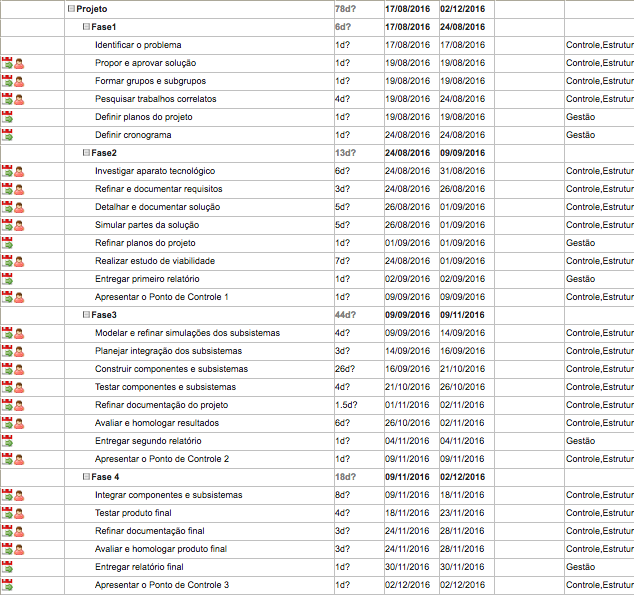
\includegraphics[scale= 0.7]{figuras/CronogramaGeral.png}
    \caption[Escopo]{Plano de Cronograma Geral do Projeto. Fonte: Autores.}
    \label{fig:cronogramaGeral}
\end{figure}

\newpage

\subsection{Cronograma de atividades do subsistema Alimentação}
A Tabela \ref{tab:cronograma_ali} apresenta todas as atividades que serão realizadas pelo subgrupo de controle até a entrega final do produto.

% ######## init table ########
\begin{table}[!htbp]
 \centering
 \caption{Cronograma de atividades do Subsistema Alimentação} \label{tab:cronograma_ali}
% distancia entre a linha e o texto
 {\renewcommand\arraystretch{1.25}
 \begin{tabular}{ l l l l l }
  \cline{1-1}\cline{2-2}\cline{3-3}\cline{4-4}\cline{5-5}  
    \multicolumn{1}{|p{6.367cm}|}{\textbf{Atividades}} &
    \multicolumn{1}{p{1.750cm}|}{\textbf{Duração}} &
    \multicolumn{1}{p{1.267cm}|}{\textbf{Data Inicial}} &
    \multicolumn{1}{p{1.233cm}|}{\textbf{Data Final}} &
    \multicolumn{1}{p{1.917cm}|}{\textbf{Status}}
  \\  
  \cline{1-1}\cline{2-2}\cline{3-3}\cline{4-4}\cline{5-5}  
    \multicolumn{1}{|p{6.367cm}|}{\textbf{Fase 1}} &
    \multicolumn{1}{p{1.750cm}|}{\textbf{7 dias}} &
    \multicolumn{1}{p{1.267cm}|}{\textbf{17/8}} &
    \multicolumn{1}{p{1.233cm}|}{\textbf{24/8}} &
    \multicolumn{1}{p{1.917cm}|}{Realizado}
  \\  
  \cline{1-1}\cline{2-2}\cline{3-3}\cline{4-4}\cline{5-5}  
    \multicolumn{1}{|p{6.367cm}|}{Realizar dimensionamento preliminar de motor elétrico} &
    \multicolumn{1}{p{1.750cm}|}{7 dias} &
    \multicolumn{1}{p{1.267cm}|}{19/8} &
    \multicolumn{1}{p{1.233cm}|}{24/8} &
    \multicolumn{1}{p{1.917cm}|}{Realizado}
  \\  
  \cline{1-1}\cline{2-2}\cline{3-3}\cline{4-4}\cline{5-5}  
    \multicolumn{1}{|p{6.367cm}|}{\textbf{Fase 2}} &
    \multicolumn{1}{p{1.750cm}|}{15 dias} &
    \multicolumn{1}{p{1.267cm}|}{\textbf{24/8}} &
    \multicolumn{1}{p{1.233cm}|}{\textbf{9/9}} &
    \multicolumn{1}{p{1.917cm}|}{Realizado}
  \\  
  \cline{1-1}\cline{2-2}\cline{3-3}\cline{4-4}\cline{5-5}  
    \multicolumn{1}{|p{6.367cm}|}{Realizar dimensionamento preliminar de bateria} &
    \multicolumn{1}{p{1.750cm}|}{5 dias} &
    \multicolumn{1}{p{1.267cm}|}{26/8} &
    \multicolumn{1}{p{1.233cm}|}{31/8} &
    \multicolumn{1}{p{1.917cm}|}{Realizado}
  \\  
  \cline{1-1}\cline{2-2}\cline{3-3}\cline{4-4}\cline{5-5}  
    \multicolumn{1}{|p{6.367cm}|}{Realizar estudo dos tipos de motor elétrico a ser utilizado} &
    \multicolumn{1}{p{1.750cm}|}{21 dias} &
    \multicolumn{1}{p{1.267cm}|}{19/9} &
    \multicolumn{1}{p{1.233cm}|}{09/9} &
    \multicolumn{1}{p{1.917cm}|}{   			

Realizado}
  \\  
  \cline{1-1}\cline{2-2}\cline{3-3}\cline{4-4}\cline{5-5}  
    \multicolumn{1}{|p{6.367cm}|}{Efetuar pesquisa de mercado para escolha do motor e bateria com as especificações definidas} &
    \multicolumn{1}{p{1.750cm}|}{14 dias} &
    \multicolumn{1}{p{1.267cm}|}{26/8} &
    \multicolumn{1}{p{1.233cm}|}{09/9} &
    \multicolumn{1}{p{1.917cm}|}{Realizado}
  \\  
  \cline{1-1}\cline{2-2}\cline{3-3}\cline{4-4}\cline{5-5}  
    \multicolumn{1}{|p{6.367cm}|}{Realizar pesquisa para otimização do torque do motor elétrico para que atinja a exigência desejada} &
    \multicolumn{1}{p{1.750cm}|}{10 dias} &
    \multicolumn{1}{p{1.267cm}|}{31/8} &
    \multicolumn{1}{p{1.233cm}|}{09/9} &
    \multicolumn{1}{p{1.917cm}|}{Realizado}
  \\  
  \cline{1-1}\cline{2-2}\cline{3-3}\cline{4-4}\cline{5-5}  
    \multicolumn{1}{|p{6.367cm}|}{Realizar pesquisa para otimização do torque do motor elétrico para que atinja a exigência desejada} &
    \multicolumn{1}{p{1.750cm}|}{10 dias} &
    \multicolumn{1}{p{1.267cm}|}{31/8} &
    \multicolumn{1}{p{1.233cm}|}{09/9} &
    \multicolumn{1}{p{1.917cm}|}{Realizado}
  \\  
  \cline{1-1}\cline{2-2}\cline{3-3}\cline{4-4}\cline{5-5}  
    \multicolumn{1}{|p{6.367cm}|}{Documentar avanços} &
    \multicolumn{1}{p{1.750cm}|}{3 dias} &
    \multicolumn{1}{p{1.267cm}|}{31/8} &
    \multicolumn{1}{p{1.233cm}|}{2/9} &
    \multicolumn{1}{p{1.917cm}|}{Realizado}
  \\  
  \cline{1-1}\cline{2-2}\cline{3-3}\cline{4-4}\cline{5-5}  
    \multicolumn{1}{|p{6.367cm}|}{Ponto de Controle 1} &
    \multicolumn{1}{p{1.750cm}|}{1 dia} &
    \multicolumn{1}{p{1.267cm}|}{9/9} &
    \multicolumn{1}{p{1.233cm}|}{9/9} &
    \multicolumn{1}{p{1.917cm}|}{Realizado}
  \\  
  \cline{1-1}\cline{2-2}\cline{3-3}\cline{4-4}\cline{5-5}  
    \multicolumn{1}{|p{6.367cm}|}{\textbf{Fase 3}} &
    \multicolumn{1}{p{1.750cm}|}{61 dias} &
    \multicolumn{1}{p{1.267cm}|}{\textbf{9/9}} &
    \multicolumn{1}{p{1.233cm}|}{\textbf{9/11}} &
    \multicolumn{1}{p{1.917cm}|}{Realizado}
  \\  
  \cline{1-1}\cline{2-2}\cline{3-3}\cline{4-4}\cline{5-5}  
    \multicolumn{1}{|p{6.367cm}|}{Escolher e comprar motores elétricos e baterias} &
    \multicolumn{1}{p{1.750cm}|}{7 dias} &
    \multicolumn{1}{p{1.267cm}|}{09/9} &
    \multicolumn{1}{p{1.233cm}|}{16/9} &
    \multicolumn{1}{p{1.917cm}|}{Realizado}
  \\  
  \cline{1-1}\cline{2-2}\cline{3-3}\cline{4-4}\cline{5-5}  
    \multicolumn{1}{|p{6.367cm}|}{Instalar motores elétricos e baterias} &
    \multicolumn{1}{p{1.750cm}|}{14 dias} &
    \multicolumn{1}{p{1.267cm}|}{26/9} &
    \multicolumn{1}{p{1.233cm}|}{10/10} &
    \multicolumn{1}{p{1.917cm}|}{Realizado}
  \\  
  \cline{1-1}\cline{2-2}\cline{3-3}\cline{4-4}\cline{5-5}  
    \multicolumn{1}{|p{6.367cm}|}{Realizar pesquisa do controlador PWM junto com a Ponte-H para controle da velocidade dos motores.em parceria com o subsistema de controle} &
    \multicolumn{1}{p{1.750cm}|}{14 dias} &
    \multicolumn{1}{p{1.267cm}|}{31/8} &
    \multicolumn{1}{p{1.233cm}|}{14/9} &
    \multicolumn{1}{p{1.917cm}|}{Realizado}
  \\  
  \cline{1-1}\cline{2-2}\cline{3-3}\cline{4-4}\cline{5-5}  
    \multicolumn{1}{|p{6.367cm}|}{Analisar a viabilidade da construção de um carregador de bateria} &
    \multicolumn{1}{p{1.750cm}|}{21 dias} &
    \multicolumn{1}{p{1.267cm}|}{09/9} &
    \multicolumn{1}{p{1.233cm}|}{30/9} &
    \multicolumn{1}{p{1.917cm}|}{Realizado}
  \\  
  \cline{1-1}\cline{2-2}\cline{3-3}\cline{4-4}\cline{5-5}  
    \multicolumn{1}{|p{6.367cm}|}{Implantar sistema de carregamento} &
    \multicolumn{1}{p{1.750cm}|}{21 dias} &
    \multicolumn{1}{p{1.267cm}|}{30/9} &
    \multicolumn{1}{p{1.233cm}|}{21/10} &
    \multicolumn{1}{p{1.917cm}|}{Realizado}
  \\  
  \cline{1-1}\cline{2-2}\cline{3-3}\cline{4-4}\cline{5-5}  
    \multicolumn{1}{|p{6.367cm}|}{Documentar avanços} &
    \multicolumn{1}{p{1.750cm}|}{2 dias} &
    \multicolumn{1}{p{1.267cm}|}{2/11} &
    \multicolumn{1}{p{1.233cm}|}{4/11} &
    \multicolumn{1}{p{1.917cm}|}{Realizado}
  \\  
  \cline{1-1}\cline{2-2}\cline{3-3}\cline{4-4}\cline{5-5}  
    \multicolumn{1}{|p{6.367cm}|}{Ponto de controle 2} &
    \multicolumn{1}{p{1.750cm}|}{1 dia} &
    \multicolumn{1}{p{1.267cm}|}{9/11} &
    \multicolumn{1}{p{1.233cm}|}{9/11} &
    \multicolumn{1}{p{1.917cm}|}{Realizado}
  \\  
  \cline{1-1}\cline{2-2}\cline{3-3}\cline{4-4}\cline{5-5}  
    \multicolumn{1}{|p{6.367cm}|}{\textbf{Fase 4}} &
    \multicolumn{1}{p{1.750cm}|}{\textbf{23 dias}} &
    \multicolumn{1}{p{1.267cm}|}{\textbf{9/11}} &
    \multicolumn{1}{p{1.233cm}|}{\textbf{2/12}} &
    \multicolumn{1}{p{1.917cm}|}{À fazer}
  \\  
  \cline{1-1}\cline{2-2}\cline{3-3}\cline{4-4}\cline{5-5}  
    \multicolumn{1}{|p{6.367cm}|}{Integrar sistema de controle de velocidade ao sistema geral} &
    \multicolumn{1}{p{1.750cm}|}{30 dias} &
    \multicolumn{1}{p{1.267cm}|}{10/10} &
    \multicolumn{1}{p{1.233cm}|}{10/11} &
    \multicolumn{1}{p{1.917cm}|}{À fazer}
  \\  
  \cline{1-1}\cline{2-2}\cline{3-3}\cline{4-4}\cline{5-5}  
    \multicolumn{1}{|p{6.367cm}|}{Testar a integração com os subsistemas – todos} &
    \multicolumn{1}{p{1.750cm}|}{12 dias} &
    \multicolumn{1}{p{1.267cm}|}{11/11} &
    \multicolumn{1}{p{1.233cm}|}{23/11} &
    \multicolumn{1}{p{1.917cm}|}{À fazer}
  \\  
  \cline{1-1}\cline{2-2}\cline{3-3}\cline{4-4}\cline{5-5}  
    \multicolumn{1}{|p{6.367cm}|}{Documentar avanços finais} &
    \multicolumn{1}{p{1.750cm}|}{5 dias} &
    \multicolumn{1}{p{1.267cm}|}{25/11} &
    \multicolumn{1}{p{1.233cm}|}{30/11} &
    \multicolumn{1}{p{1.917cm}|}{À fazer}
  \\  
  \cline{1-1}\cline{2-2}\cline{3-3}\cline{4-4}\cline{5-5}  
    \multicolumn{1}{|p{6.367cm}|}{Apresentação final} &
    \multicolumn{1}{p{1.750cm}|}{1 dia} &
    \multicolumn{1}{p{1.267cm}|}{2/12} &
    \multicolumn{1}{p{1.233cm}|}{2/12} &
    \multicolumn{1}{p{1.917cm}|}{À fazer}
  \\  
  \hline

 \end{tabular} }
\end{table}

\newpage

\subsection{Cronograma de atividades do subsistema Estrutura}

A Tabela a seguir apresenta todas as atividades que serão realizadas pelo subgrupo de estrutura até a entrega final do produto.

% ######## init table ########
\begin{table}[H]
 \centering
% distancia entre a linha e o texto
 {\renewcommand\arraystretch{1.25}
 \label{tab:cronestr}
 \caption{Cronograma de atividades Estrutura.}
 \begin{tabular}{ l l l l l }
  \cline{1-1}\cline{2-2}\cline{3-3}\cline{4-4}\cline{5-5}  
    \multicolumn{1}{|p{3.867cm}|}{\textbf{Atividade} \centering } &
    \multicolumn{1}{p{1.700cm}|}{\textbf{Duração} \centering } &
    \multicolumn{1}{p{1.133cm}|}{\textbf{Data inicial} \centering } &
    \multicolumn{1}{p{0.967cm}|}{\textbf{Data Final} \centering } &
    \multicolumn{1}{p{1.833cm}|}{\textbf{Status} \centering }
  \\  
  \cline{1-1}\cline{2-2}\cline{3-3}\cline{4-4}\cline{5-5}  
    \multicolumn{1}{|p{3.867cm}|}{Fase 1} &
    \multicolumn{1}{p{1.700cm}|}{7 dias \centering } &
    \multicolumn{1}{p{1.133cm}|}{17/08 \centering } &
    \multicolumn{1}{p{0.967cm}|}{24/08 \centering } &
    \multicolumn{1}{p{1.833cm}|}{Realizado \centering }
  \\  
  \cline{1-1}\cline{2-2}\cline{3-3}\cline{4-4}\cline{5-5}  
    \multicolumn{1}{|p{3.867cm}|}{Definir a geometria do carrinho} &
    \multicolumn{1}{p{1.700cm}|}{1 dia \centering } &
    \multicolumn{1}{p{1.133cm}|}{19/08 \centering } &
    \multicolumn{1}{p{0.967cm}|}{19/08 \centering } &
    \multicolumn{1}{p{1.833cm}|}{Realizado \centering }
  \\  
  \cline{1-1}\cline{2-2}\cline{3-3}\cline{4-4}\cline{5-5}  
    \multicolumn{1}{|p{3.867cm}|}{Pesquisa de ergonimia} &
    \multicolumn{1}{p{1.700cm}|}{5 dias \centering } &
    \multicolumn{1}{p{1.133cm}|}{19/08 \centering } &
    \multicolumn{1}{p{0.967cm}|}{24/08 \centering } &
    \multicolumn{1}{p{1.833cm}|}{Realizado \centering }
  \\  
  \cline{1-1}\cline{2-2}\cline{3-3}\cline{4-4}\cline{5-5}  
    \multicolumn{1}{|p{3.867cm}|}{Pesquisa de material } &
    \multicolumn{1}{p{1.700cm}|}{5 dias \centering } &
    \multicolumn{1}{p{1.133cm}|}{ 19/08 \centering } &
    \multicolumn{1}{p{0.967cm}|}{24/08 \centering } &
    \multicolumn{1}{p{1.833cm}|}{Realizado \centering }
  \\  
  \cline{1-1}\cline{2-2}\cline{3-3}\cline{4-4}\cline{5-5}  
    \multicolumn{1}{|p{3.867cm}|}{Definir componentes estruturais} &
    \multicolumn{1}{p{1.700cm}|}{5 dias \centering } &
    \multicolumn{1}{p{1.133cm}|}{19/08 \centering } &
    \multicolumn{1}{p{0.967cm}|}{24/08 \centering } &
    \multicolumn{1}{p{1.833cm}|}{Realizado \centering }
  \\  
  \cline{1-1}\cline{2-2}\cline{3-3}\cline{4-4}\cline{5-5}  
    \multicolumn{1}{|p{3.867cm}|}{Definir cronograma} &
    \multicolumn{1}{p{1.700cm}|}{1 dia \centering } &
    \multicolumn{1}{p{1.133cm}|}{24/08 \centering } &
    \multicolumn{1}{p{0.967cm}|}{24/08 \centering } &
    \multicolumn{1}{p{1.833cm}|}{Realizado \centering }
  \\  
  \cline{1-1}\cline{2-2}\cline{3-3}\cline{4-4}\cline{5-5}  
    \multicolumn{1}{|p{3.867cm}|}{Fase 2} &
    \multicolumn{1}{p{1.700cm}|}{15 dias \centering } &
    \multicolumn{1}{p{1.133cm}|}{24/08 \centering } &
    \multicolumn{1}{p{0.967cm}|}{09/09 \centering } &
    \multicolumn{1}{p{1.833cm}|}{Realizado \centering }
  \\  
  \cline{1-1}\cline{2-2}\cline{3-3}\cline{4-4}\cline{5-5}  
    \multicolumn{1}{|p{3.867cm}|}{Fazer CAD inicial do carrinho} &
    \multicolumn{1}{p{1.700cm}|}{5 dias \centering } &
    \multicolumn{1}{p{1.133cm}|}{26/08 \centering } &
    \multicolumn{1}{p{0.967cm}|}{31/08 \centering } &
    \multicolumn{1}{p{1.833cm}|}{Realizado \centering }
  \\  
  \cline{1-1}\cline{2-2}\cline{3-3}\cline{4-4}\cline{5-5}  
    \multicolumn{1}{|p{3.867cm}|}{Pesquisa de modelo de rodinhas, transmissão e custos} &
    \multicolumn{1}{p{1.700cm}|}{5 dias \centering } &
    \multicolumn{1}{p{1.133cm}|}{26/08 \centering } &
    \multicolumn{1}{p{0.967cm}|}{31/08 \centering } &
    \multicolumn{1}{p{1.833cm}|}{Realizado \centering }
  \\  
  \cline{1-1}\cline{2-2}\cline{3-3}\cline{4-4}\cline{5-5}  
    \multicolumn{1}{|p{3.867cm}|}{Documentação} &
    \multicolumn{1}{p{1.700cm}|}{3 dis \centering } &
    \multicolumn{1}{p{1.133cm}|}{29/08 \centering } &
    \multicolumn{1}{p{0.967cm}|}{02/09 \centering } &
    \multicolumn{1}{p{1.833cm}|}{Realizado \centering }
  \\  
  \cline{1-1}\cline{2-2}\cline{3-3}\cline{4-4}\cline{5-5}  
    \multicolumn{1}{|p{3.867cm}|}{Apresentação} &
    \multicolumn{1}{p{1.700cm}|}{1 dia \centering } &
    \multicolumn{1}{p{1.133cm}|}{09/09 \centering } &
    \multicolumn{1}{p{0.967cm}|}{09/09 \centering } &
    \multicolumn{1}{p{1.833cm}|}{Realizado \centering }
  \\  
  \cline{1-1}\cline{2-2}\cline{3-3}\cline{4-4}\cline{5-5}  
    \multicolumn{1}{|p{3.867cm}|}{Fase 3} &
    \multicolumn{1}{p{1.700cm}|}{61 dias \centering } &
    \multicolumn{1}{p{1.133cm}|}{09/09 \centering } &
    \multicolumn{1}{p{0.967cm}|}{09/11 \centering } &
    \multicolumn{1}{p{1.833cm}|}{Realizado \centering }
  \\  
  \cline{1-1}\cline{2-2}\cline{3-3}\cline{4-4}\cline{5-5}  
    \multicolumn{1}{|p{3.867cm}|}{Pesquisa de processos de fabricação} &
    \multicolumn{1}{p{1.700cm}|}{5 dias \centering } &
    \multicolumn{1}{p{1.133cm}|}{09/09 \centering } &
    \multicolumn{1}{p{0.967cm}|}{14/09 \centering } &
    \multicolumn{1}{p{1.833cm}|}{Realizado \centering }
  \\  
  \cline{1-1}\cline{2-2}\cline{3-3}\cline{4-4}\cline{5-5}  
    \multicolumn{1}{|p{3.867cm}|}{Definir modelos de rodas e transmissão} &
    \multicolumn{1}{p{1.700cm}|}{12 dias \centering } &
    \multicolumn{1}{p{1.133cm}|}{02/09 \centering } &
    \multicolumn{1}{p{0.967cm}|}{14/09 \centering } &
    \multicolumn{1}{p{1.833cm}|}{Realizado \centering }
  \\  
  \cline{1-1}\cline{2-2}\cline{3-3}\cline{4-4}\cline{5-5}  
    \multicolumn{1}{|p{3.867cm}|}{Cálculos de transmissão} &
    \multicolumn{1}{p{1.700cm}|}{7 dias \centering } &
    \multicolumn{1}{p{1.133cm}|}{14/09 \centering } &
    \multicolumn{1}{p{0.967cm}|}{21/09 \centering } &
    \multicolumn{1}{p{1.833cm}|}{Realizado \centering }
  \\  
  \cline{1-1}\cline{2-2}\cline{3-3}\cline{4-4}\cline{5-5}  
    \multicolumn{1}{|p{3.867cm}|}{Pesquisa de mercado de transmissão e material} &
    \multicolumn{1}{p{1.700cm}|}{3 dias \centering } &
    \multicolumn{1}{p{1.133cm}|}{21/09 \centering } &
    \multicolumn{1}{p{0.967cm}|}{23/09 \centering } &
    \multicolumn{1}{p{1.833cm}|}{Realizado \centering }
  \\  
  \cline{1-1}\cline{2-2}\cline{3-3}\cline{4-4}\cline{5-5}  
    \multicolumn{1}{|p{3.867cm}|}{Simulação do CAD} &
    \multicolumn{1}{p{1.700cm}|}{11 dias \centering } &
    \multicolumn{1}{p{1.133cm}|}{28/09 \centering } &
    \multicolumn{1}{p{0.967cm}|}{07/10 \centering } &
    \multicolumn{1}{p{1.833cm}|}{Realizado \centering }
  \\  
  \cline{1-1}\cline{2-2}\cline{3-3}\cline{4-4}\cline{5-5}  
    \multicolumn{1}{|p{3.867cm}|}{Compra de recursos (material, rodinhas e transmissão)} &
    \multicolumn{1}{p{1.700cm}|}{8 dias \centering } &
    \multicolumn{1}{p{1.133cm}|}{30/09 \centering } &
    \multicolumn{1}{p{0.967cm}|}{07/10 \centering } &
    \multicolumn{1}{p{1.833cm}|}{Realizado \centering }
  \\  
  \cline{1-1}\cline{2-2}\cline{3-3}\cline{4-4}\cline{5-5}  
    \multicolumn{1}{|p{3.867cm}|}{Fabricação da estrutura e de suporte} &
    \multicolumn{1}{p{1.700cm}|}{17 dias \centering } &
    \multicolumn{1}{p{1.133cm}|}{21/10 \centering } &
    \multicolumn{1}{p{0.967cm}|}{28/10 \centering } &
    \multicolumn{1}{p{1.833cm}|}{Realizado \centering }
  \\  
  \cline{1-1}\cline{2-2}\cline{3-3}\cline{4-4}\cline{5-5}  
    \multicolumn{1}{|p{3.867cm}|}{Documentação dos avanços} &
    \multicolumn{1}{p{1.700cm}|}{5 dias \centering } &
    \multicolumn{1}{p{1.133cm}|}{21/10 \centering } &
    \multicolumn{1}{p{0.967cm}|}{28/10 \centering } &
    \multicolumn{1}{p{1.833cm}|}{Realizado \centering }
  \\  
  \cline{1-1}\cline{2-2}\cline{3-3}\cline{4-4}\cline{5-5}  
    \multicolumn{1}{|p{3.867cm}|}{Apresentação} &
    \multicolumn{1}{p{1.700cm}|}{1 dia \centering } &
    \multicolumn{1}{p{1.133cm}|}{09/11 \centering } &
    \multicolumn{1}{p{0.967cm}|}{09/11 \centering } &
    \multicolumn{1}{p{1.833cm}|}{Realizado \centering }
  \\  
  \cline{1-1}\cline{2-2}\cline{3-3}\cline{4-4}\cline{5-5}  
    \multicolumn{1}{|p{3.867cm}|}{Fase 4} &
    \multicolumn{1}{p{1.700cm}|}{23 dias \centering } &
    \multicolumn{1}{p{1.133cm}|}{09/11 \centering } &
    \multicolumn{1}{p{0.967cm}|}{02/12 \centering } &
    \multicolumn{1}{p{1.833cm}|}{À fazer \centering }
  \\  
  \cline{1-1}\cline{2-2}\cline{3-3}\cline{4-4}\cline{5-5}  
    \multicolumn{1}{|p{3.867cm}|}{Integração dos subsistemas} &
    \multicolumn{1}{p{1.700cm}|}{12 dias \centering } &
    \multicolumn{1}{p{1.133cm}|}{11/11 \centering } &
    \multicolumn{1}{p{0.967cm}|}{30/11 \centering } &
    \multicolumn{1}{p{1.833cm}|}{À fazer \centering }
  \\  
  \cline{1-1}\cline{2-2}\cline{3-3}\cline{4-4}\cline{5-5}  
    \multicolumn{1}{|p{3.867cm}|}{Documentação final} &
    \multicolumn{1}{p{1.700cm}|}{5 dias \centering } &
    \multicolumn{1}{p{1.133cm}|}{25/11 \centering } &
    \multicolumn{1}{p{0.967cm}|}{30/11 \centering } &
    \multicolumn{1}{p{1.833cm}|}{À fazer \centering }
  \\  
  \cline{1-1}\cline{2-2}\cline{3-3}\cline{4-4}\cline{5-5}  
    \multicolumn{1}{|p{3.867cm}|}{Apresentação final} &
    \multicolumn{1}{p{1.700cm}|}{1 dia \centering } &
    \multicolumn{1}{p{1.133cm}|}{02/10 \centering } &
    \multicolumn{1}{p{0.967cm}|}{02/12 \centering } &
    \multicolumn{1}{p{1.833cm}|}{À fazer \centering }
  \\  
  \hline

 \end{tabular} }
\end{table}

\newpage

\subsection{Cronograma de atividades do subsistema Controle}

A Tabela \ref{tab:cronograma_controle} apresenta todas as atividades que serão realizadas pelo subgrupo de controle até a entrega final do produto.

% ######## init table ########
\begin{table}[!htbp]
 \centering
 \caption{Cronograma de atividades do Subsistema Controle} \label{tab:cronograma_controle}
% distancia entre a linha e o texto
 {\renewcommand\arraystretch{1.25}
 \begin{tabular}{ l l l l l }
  \cline{1-1}\cline{2-2}\cline{3-3}\cline{4-4}\cline{5-5}  
    \multicolumn{1}{|p{6.900cm}|}{\textbf{Atividades}} &
    \multicolumn{1}{p{1.817cm}|}{\textbf{Duração}} &
    \multicolumn{1}{p{1.650cm}|}{\textbf{Data de início}} &
    \multicolumn{1}{p{1.550cm}|}{\textbf{Data de fim}} &
    \multicolumn{1}{p{2.000cm}|}{\textbf{Status}}
  \\  
  \cline{1-1}\cline{2-2}\cline{3-3}\cline{4-4}\cline{5-5}  
    \multicolumn{1}{|p{6.900cm}|}{\textbf{Fase 1}} &
    \multicolumn{1}{p{1.817cm}|}{\textbf{7 dias}} &
    \multicolumn{1}{p{1.650cm}|}{\textbf{17/08}} &
    \multicolumn{1}{p{1.550cm}|}{\textbf{24/08}} &
    \multicolumn{1}{p{2.000cm}|}{\textbf{Realizado}}
  \\  
  \cline{1-1}\cline{2-2}\cline{3-3}\cline{4-4}\cline{5-5}  
    \multicolumn{1}{|p{6.900cm}|}{Pesquisar trabalhos correlatos} &
    \multicolumn{1}{p{1.817cm}|}{5 dias} &
    \multicolumn{1}{p{1.650cm}|}{19/08} &
    \multicolumn{1}{p{1.550cm}|}{24/08} &
    \multicolumn{1}{p{2.000cm}|}{Realizado}
  \\  
  \cline{1-1}\cline{2-2}\cline{3-3}\cline{4-4}\cline{5-5}  
    \multicolumn{1}{|p{6.900cm}|}{Definir cronograma de controle} &
    \multicolumn{1}{p{1.817cm}|}{1 dia} &
    \multicolumn{1}{p{1.650cm}|}{24/8} &
    \multicolumn{1}{p{1.550cm}|}{24/8} &
    \multicolumn{1}{p{2.000cm}|}{Realizado}
  \\  
  \cline{1-1}\cline{2-2}\cline{3-3}\cline{4-4}\cline{5-5}  
    \multicolumn{1}{|p{6.900cm}|}{\textbf{Fase 2}} &
    \multicolumn{1}{p{1.817cm}|}{\textbf{15 dias}} &
    \multicolumn{1}{p{1.650cm}|}{\textbf{24/8}} &
    \multicolumn{1}{p{1.550cm}|}{\textbf{9/9}} &
    \multicolumn{1}{p{2.000cm}|}{Realizado}
  \\  
  \cline{1-1}\cline{2-2}\cline{3-3}\cline{4-4}\cline{5-5}  
    \multicolumn{1}{|p{6.900cm}|}{Propor um esquema de solução} &
    \multicolumn{1}{p{1.817cm}|}{1 dia} &
    \multicolumn{1}{p{1.650cm}|}{24/8} &
    \multicolumn{1}{p{1.550cm}|}{24/8} &
    \multicolumn{1}{p{2.000cm}|}{Realizado}
  \\  
  \cline{1-1}\cline{2-2}\cline{3-3}\cline{4-4}\cline{5-5}  
    \multicolumn{1}{|p{6.900cm}|}{Pesquisar componentes do esquema  			

Sensores e processadores – eletrônica  			

Algoritmos - software} &
    \multicolumn{1}{p{1.817cm}|}{2 dias} &
    \multicolumn{1}{p{1.650cm}|}{24/08} &
    \multicolumn{1}{p{1.550cm}|}{26/8} &
    \multicolumn{1}{p{2.000cm}|}{Realizado}
  \\  
  \cline{1-1}\cline{2-2}\cline{3-3}\cline{4-4}\cline{5-5}  
    \multicolumn{1}{|p{6.900cm}|}{Projetar montagem e fabricação} &
    \multicolumn{1}{p{1.817cm}|}{1 dia} &
    \multicolumn{1}{p{1.650cm}|}{31/8} &
    \multicolumn{1}{p{1.550cm}|}{31/8} &
    \multicolumn{1}{p{2.000cm}|}{Realizado}
  \\  
  \cline{1-1}\cline{2-2}\cline{3-3}\cline{4-4}\cline{5-5}  
    \multicolumn{1}{|p{6.900cm}|}{Escrever relatório} &
    \multicolumn{1}{p{1.817cm}|}{3 dias} &
    \multicolumn{1}{p{1.650cm}|}{31/8} &
    \multicolumn{1}{p{1.550cm}|}{2/9} &
    \multicolumn{1}{p{2.000cm}|}{Realizado}
  \\  
  \cline{1-1}\cline{2-2}\cline{3-3}\cline{4-4}\cline{5-5}  
    \multicolumn{1}{|p{6.900cm}|}{Apresentação - todos} &
    \multicolumn{1}{p{1.817cm}|}{1 dia} &
    \multicolumn{1}{p{1.650cm}|}{9/9} &
    \multicolumn{1}{p{1.550cm}|}{9/9} &
    \multicolumn{1}{p{2.000cm}|}{Realizado}
  \\  
  \cline{1-1}\cline{2-2}\cline{3-3}\cline{4-4}\cline{5-5}  
    \multicolumn{1}{|p{6.900cm}|}{\textbf{Fase 3}} &
    \multicolumn{1}{p{1.817cm}|}{\textbf{61 dias}} &
    \multicolumn{1}{p{1.650cm}|}{\textbf{9/9}} &
    \multicolumn{1}{p{1.550cm}|}{\textbf{9/11}} &
    \multicolumn{1}{p{2.000cm}|}{\textbf{Realizado}}
  \\  
  \cline{1-1}\cline{2-2}\cline{3-3}\cline{4-4}\cline{5-5}  
    \multicolumn{1}{|p{6.900cm}|}{Definir e escolher componentes a - eletrônica} &
    \multicolumn{1}{p{1.817cm}|}{6 dias} &
    \multicolumn{1}{p{1.650cm}|}{14/9} &
    \multicolumn{1}{p{1.550cm}|}{20/9} &
    \multicolumn{1}{p{2.000cm}|}{Realizado}
  \\  
  \cline{1-1}\cline{2-2}\cline{3-3}\cline{4-4}\cline{5-5}  
    \multicolumn{1}{|p{6.900cm}|}{Definir algoritmos utilizados – software} &
    \multicolumn{1}{p{1.817cm}|}{6 dias} &
    \multicolumn{1}{p{1.650cm}|}{14/9} &
    \multicolumn{1}{p{1.550cm}|}{20/9} &
    \multicolumn{1}{p{2.000cm}|}{Realizado}
  \\  
  \cline{1-1}\cline{2-2}\cline{3-3}\cline{4-4}\cline{5-5}  
    \multicolumn{1}{|p{6.900cm}|}{Realizar simulações das placas projetadas – eletrônica} &
    \multicolumn{1}{p{1.817cm}|}{3 dias} &
    \multicolumn{1}{p{1.650cm}|}{20/9} &
    \multicolumn{1}{p{1.550cm}|}{23/9} &
    \multicolumn{1}{p{2.000cm}|}{Realizado}
  \\  
  \cline{1-1}\cline{2-2}\cline{3-3}\cline{4-4}\cline{5-5}  
    \multicolumn{1}{|p{6.900cm}|}{Testar de algoritmo em primeiro protótipo – software} &
    \multicolumn{1}{p{1.817cm}|}{30 dias} &
    \multicolumn{1}{p{1.650cm}|}{23/9} &
    \multicolumn{1}{p{1.550cm}|}{21/10} &
    \multicolumn{1}{p{2.000cm}|}{Realizado}
  \\  
  \cline{1-1}\cline{2-2}\cline{3-3}\cline{4-4}\cline{5-5}  
    \multicolumn{1}{|p{6.900cm}|}{Confeccionar placas – eletrônica} &
    \multicolumn{1}{p{1.817cm}|}{16 dias} &
    \multicolumn{1}{p{1.650cm}|}{4 /10} &
    \multicolumn{1}{p{1.550cm}|}{21/10} &
    \multicolumn{1}{p{2.000cm}|}{Realizado}
  \\  
  \cline{1-1}\cline{2-2}\cline{3-3}\cline{4-4}\cline{5-5}  
    \multicolumn{1}{|p{6.900cm}|}{Testar placas – eletrônica} &
    \multicolumn{1}{p{1.817cm}|}{3 dias} &
    \multicolumn{1}{p{1.650cm}|}{25/10} &
    \multicolumn{1}{p{1.550cm}|}{28/10} &
    \multicolumn{1}{p{2.000cm}|}{Realizado}
  \\  
  \cline{1-1}\cline{2-2}\cline{3-3}\cline{4-4}\cline{5-5}  
    \multicolumn{1}{|p{6.900cm}|}{Projetar a integração com outros subsistemas - todos} &
    \multicolumn{1}{p{1.817cm}|}{3 dias} &
    \multicolumn{1}{p{1.650cm}|}{25/10} &
    \multicolumn{1}{p{1.550cm}|}{28/10} &
    \multicolumn{1}{p{2.000cm}|}{Realizado}
  \\  
  \cline{1-1}\cline{2-2}\cline{3-3}\cline{4-4}\cline{5-5}  
    \multicolumn{1}{|p{6.900cm}|}{Documentar avanços} &
    \multicolumn{1}{p{1.817cm}|}{2 dias} &
    \multicolumn{1}{p{1.650cm}|}{2/11} &
    \multicolumn{1}{p{1.550cm}|}{4/11} &
    \multicolumn{1}{p{2.000cm}|}{Realizado}
  \\  
  \cline{1-1}\cline{2-2}\cline{3-3}\cline{4-4}\cline{5-5}  
    \multicolumn{1}{|p{6.900cm}|}{Apresentação – todos} &
    \multicolumn{1}{p{1.817cm}|}{1 dia} &
    \multicolumn{1}{p{1.650cm}|}{9/11} &
    \multicolumn{1}{p{1.550cm}|}{9/11} &
    \multicolumn{1}{p{2.000cm}|}{À fazer}
  \\  
  \cline{1-1}\cline{2-2}\cline{3-3}\cline{4-4}\cline{5-5}  
    \multicolumn{1}{|p{6.900cm}|}{\textbf{Fase 4}} &
    \multicolumn{1}{p{1.817cm}|}{\textbf{23 dias}} &
    \multicolumn{1}{p{1.650cm}|}{\textbf{9/11}} &
    \multicolumn{1}{p{1.550cm}|}{\textbf{2/12}} &
    \multicolumn{1}{p{2.000cm}|}{À fazer}
  \\  
  \cline{1-1}\cline{2-2}\cline{3-3}\cline{4-4}\cline{5-5}  
    \multicolumn{1}{|p{6.900cm}|}{Testar a integração com os subsistemas} &
    \multicolumn{1}{p{1.817cm}|}{12 dias} &
    \multicolumn{1}{p{1.650cm}|}{11/11} &
    \multicolumn{1}{p{1.550cm}|}{23/11} &
    \multicolumn{1}{p{2.000cm}|}{À fazer}
  \\  
  \cline{1-1}\cline{2-2}\cline{3-3}\cline{4-4}\cline{5-5}  
    \multicolumn{1}{|p{6.900cm}|}{Definir o protótipo final} &
    \multicolumn{1}{p{1.817cm}|}{5 dias} &
    \multicolumn{1}{p{1.650cm}|}{25/11} &
    \multicolumn{1}{p{1.550cm}|}{30/11} &
    \multicolumn{1}{p{2.000cm}|}{À fazer}
  \\  
  \cline{1-1}\cline{2-2}\cline{3-3}\cline{4-4}\cline{5-5}  
    \multicolumn{1}{|p{6.900cm}|}{Documentar avanços finais} &
    \multicolumn{1}{p{1.817cm}|}{5 dias} &
    \multicolumn{1}{p{1.650cm}|}{25/11} &
    \multicolumn{1}{p{1.550cm}|}{30/11} &
    \multicolumn{1}{p{2.000cm}|}{À fazer}
  \\  
  \cline{1-1}\cline{2-2}\cline{3-3}\cline{4-4}\cline{5-5}  
    \multicolumn{1}{|p{6.900cm}|}{Apresentação final} &
    \multicolumn{1}{p{1.817cm}|}{1 dia} &
    \multicolumn{1}{p{1.650cm}|}{2/12} &
    \multicolumn{1}{p{1.550cm}|}{2/12} &
    \multicolumn{1}{p{2.000cm}|}{À fazer}
  \\  
  \hline

 \end{tabular} }
\end{table}


\subsubsection{Controle do tempo e mudanças}

O desenvolvimento de cada tarefa do cronograma é designada a pelo menos um dos integrantes do grupo de acordo com a sua afinidade com a atividade e disponibilidade. Cada membro é responsável por atualizar o status de suas atividades no cronograma do projeto.

Todas as possíveis mudanças no projeto serão analisadas pelo grupo, pois uma mudança pode afetar o escopo, tempo e custo do projeto. O time irá reagir a esta mudança decidindo se esta irá ser desenvolvida ou não seguindo os planos de gerenciamento de escopo e riscos do projeto.

Caso a mudança seja aceita isto refletirá no cronograma e a equipe de gestão será responsável em acomodar a mudança. Caso a mudança seja inevitável, a equipe deve moldar as atividades do cronograma para minimizar ao máximo os impactos negativos de tal mudança.

\section{Custos}

\subsection{Custo de recursos humanos} \label{subsec:custos_rh}

O projeto será desenvolvido por treze alunos da disciplina "Projeto Integrador 2" dos cursos de graduação da Universidade de Brasília - Faculdade UnB Gama. Baseado no Relatório de Gestão 2015 da Universidade de Brasília \cite{unb2015}, um aluno custou R\textdollar{ 16.640,00} no ano de 2015 Considerando que um ano letivo tem 200 dias, podemos calcular um custo de aluno como sendo de R\textdollar{ 83,20} por dia. Considere que a média de créditos que um aluno cursa por semestre como(máximo de créditos + mínimo de créditos)/2 = 24. 

Com esse valor podemos deduzir que o média de quantidade de horas por dia de um aluno é 5h. Sendo assim podemos deduzir que o preço do aluno por hora é de R\textdollar{  16,64}.
Levando esses dados em conta e considerando que um aluno trabalhe 8h por semana no projeto, o aluno custará: R\textdollar{ 133,12} por semana.
Considerando que o projeto tem aproximadamente 16 semanas temos um custo de R\textdollar{  2.129,00} por aluno. O projeto possui 13 alunos, então o custo total pela mão de obra dos alunos do projeto é de R\textdollar{27.688,96}.



\subsection{Custo dos recursos materiais}
O grupo fez um levantamento inicial dos materiais necessários para a realização do projeto. Assim como todo projeto, os custos também foram divididos em subáreas. A Tabela \ref{tab:custo_sub} organiza os custos para cada subsistema do projteto:


% ######## init table ########
\begin{table}[h]
 \centering
 \caption{Custos dos subsistemas} \label{tab:custo_sub}
% distancia entre a linha e o texto
 {\renewcommand\arraystretch{1.25}
 \begin{tabular}{ l l }
  \cline{1-1}\cline{2-2}  
    \multicolumn{1}{|c|}{\textbf{Subsistema}} &
    \multicolumn{1}{c|}{\textbf{Custo Estimado}}
  \\  
  \cline{1-1}\cline{2-2}  
    \multicolumn{1}{|c|}{Alimentação} &
    \multicolumn{1}{c|}{R\$ 830,00}
  \\  
  \cline{1-1}\cline{2-2}  
    \multicolumn{1}{|c|}{Estrutura} &
    \multicolumn{1}{c|}{R\$ 300,00}
  \\  
  \cline{1-1}\cline{2-2}  
    \multicolumn{1}{|c|}{Controle} &
    \multicolumn{1}{c|}{R\$ 665,00}
  \\  
  \cline{1-1}\cline{2-2}  
    \multicolumn{1}{|c|}{\textbf{Total}} &
    \multicolumn{1}{c|}{R\$ 1.795,00}
  \\  
  \hline

 \end{tabular} }
\end{table}

Esses valores podem sofrer alterações até o fim do projeto. Entretanto este é o custo estimado inicial de recursos materiais.

\subsection{Cronograma físico-financeiro do subsistema Alimentação}

Os custos referentes ao subsistema Alimentação é apresentado na Tabela \ref{tab:custo_alimentacao}. 

% ######## init table ########
\begin{table}[h]
 \centering
% distancia entre a linha e o texto
 {\renewcommand\arraystretch{1.25}
 \caption{Crononograma físico-financeiro do subsistema Alimentação.}
 \label{tab:custo_alimentacao}
 \begin{tabular}{ l l l }
  \cline{1-1}\cline{2-2}\cline{3-3}  
    \multicolumn{1}{|c|}{\textbf{Recurso} \centering } &
    \multicolumn{1}{c|}{\textbf{Data de aquisição} \centering } &
    \multicolumn{1}{c|}{\textbf{Estimativa de preço} \centering }
  \\  
  \cline{1-1}\cline{2-2}\cline{3-3}  
    \multicolumn{1}{|p{3.850cm}|}{Motor elétrico \centering } &
    \multicolumn{1}{p{4.217cm}|}{20/09 a 30/09/2016 \centering } &
    \multicolumn{1}{p{4.217cm}|}{R\$ 200,00 \centering }
  \\  
  \cline{1-1}\cline{2-2}\cline{3-3}  
    \multicolumn{1}{|p{3.850cm}|}{Bateria \centering } &
    \multicolumn{1}{p{4.217cm}|}{05/09 a 18/09/2016 \centering } &
    \multicolumn{1}{p{4.217cm}|}{R\$ 400,00 \centering }
  \\  
  \cline{1-1}\cline{2-2}\cline{3-3}  
    \multicolumn{1}{|p{3.850cm}|}{Materiais para o carregador da bateria \centering } &
    \multicolumn{1}{p{4.217cm}|}{15/10 a 30/10/2016 \centering } &
    \multicolumn{1}{p{4.217cm}|}{R\$ 200,00 \centering }
  \\  
  \cline{1-1}\cline{2-2}\cline{3-3}  
    \multicolumn{2}{|p{3.850cm}|}{Total \centering } &
    \multicolumn{1}{p{4.217cm}|}{R\$ 800,00 \centering }
  \\  
  \hline

 \end{tabular} }
\end{table}




\subsection{Cronograma físico-financeiro do subsistema Estrutura}

A estimativa de preços e aquisição para os recursos de estrutura foram estimados na Tabela \ref{tab:custos_estrutura}.

% ######## init table ########
\begin{table}[h]
 \centering
% distancia entre a linha e o texto
 {\renewcommand\arraystretch{1.25}
 \caption{Crononograma físico-financeiro Estrutura.}
 \label{tab:custos_estrutura}
 \begin{tabular}{ l l l }
  \cline{1-1}\cline{2-2}\cline{3-3}  
    \multicolumn{1}{|c|}{\textbf{Recurso} \centering } &
    \multicolumn{1}{c|}{\textbf{Data de aquisição} \centering } &
    \multicolumn{1}{c|}{\textbf{Estimativa de preço} \centering }
  \\  
  \cline{1-1}\cline{2-2}\cline{3-3}  
    \multicolumn{1}{|p{3.850cm}|}{Material para estrutura \centering } &
    \multicolumn{1}{p{4.217cm}|}{30/09 a 07/10/2016 \centering } &
    \multicolumn{1}{p{4.217cm}|}{R\$ 50,00 \centering }
  \\  
  \cline{1-1}\cline{2-2}\cline{3-3}  
    \multicolumn{1}{|p{3.850cm}|}{Rodas \centering } &
    \multicolumn{1}{p{4.217cm}|}{30/09 a 07/10/2016 \centering } &
    \multicolumn{1}{p{4.217cm}|}{R\$ 150,00 \centering }
  \\  
  \cline{1-1}\cline{2-2}\cline{3-3}  
    \multicolumn{1}{|p{3.850cm}|}{Trasmissão \centering } &
    \multicolumn{1}{p{4.217cm}|}{30/09 a 07/10/2016 \centering } &
    \multicolumn{1}{p{4.217cm}|}{R\$ 100,00 \centering }
  \\  
  \cline{1-1}\cline{2-2}\cline{3-3}  
    \multicolumn{2}{|p{3.850cm}|}{Total \centering } &
    \multicolumn{1}{p{4.217cm}|}{R\$ 300,00 \centering }
  \\  
  \hline

 \end{tabular} }
\end{table}

\subsection{Cronograma físico-financeiro do subsistema Controle}
Para o projeto do subsistema Controle e Automação, foi feita uma estimativa de tempo de aquisição e preços possíveis dos componentes desse subproduto.

% ######## init table ########
\begin{table}[h]
 \centering
% distancia entre a linha e o texto
 {\renewcommand\arraystretch{1.25}
 \caption{Cronograma custo-financeiro Controle.}
 \begin{tabular}{ l l l }
  \cline{1-1}\cline{2-2}\cline{3-3}  
    \multicolumn{1}{|c|}{\textbf{Componentes/Recursos} \centering } &
    \multicolumn{1}{c|}{\textbf{Data de aquisição} \centering } &
    \multicolumn{1}{c|}{\textbf{Estimativa de preço} \centering }
  \\  
  \cline{1-1}\cline{2-2}\cline{3-3}  
    \multicolumn{1}{|p{3.850cm}|}{Microprocessador (CPU) \centering } &
    \multicolumn{1}{p{4.217cm}|}{14/09 a 4/10/2016 \centering } &
    \multicolumn{1}{p{4.217cm}|}{R\$ 25,00 \centering }
  \\  
  \cline{1-1}\cline{2-2}\cline{3-3}  
    \multicolumn{1}{|p{3.850cm}|}{Sensores \centering } &
    \multicolumn{1}{p{4.217cm}|}{14/09 a 4/10/2016 \centering } &
    \multicolumn{1}{p{4.217cm}|}{R\$ 30,00 \centering }
  \\  
  \cline{1-1}\cline{2-2}\cline{3-3}  
    \multicolumn{1}{|p{3.850cm}|}{Ponte h \centering } &
    \multicolumn{1}{p{4.217cm}|}{14/09 a 4/10/2016 \centering } &
    \multicolumn{1}{p{4.217cm}|}{R\$ 50,00 \centering }
  \\  
  \cline{1-1}\cline{2-2}\cline{3-3}  
    \multicolumn{1}{|p{3.850cm}|}{Raspberry Pi  \centering } &
    \multicolumn{1}{p{4.217cm}|}{14/09 a 4/10/2016 \centering } &
    \multicolumn{1}{p{4.217cm}|}{R\$ 300.00 \centering }
  \\  
  \cline{1-1}\cline{2-2}\cline{3-3}  
    \multicolumn{1}{|p{3.850cm}|}{Codificador e Decofificador RF \centering } &
    \multicolumn{1}{p{4.217cm}|}{14/09 a 4/10/2016 \centering } &
    \multicolumn{1}{p{4.217cm}|}{R\$ 40,00 \centering }
  \\  
  \cline{1-1}\cline{2-2}\cline{3-3}  
    \multicolumn{1}{|p{3.850cm}|}{Antena \centering } &
    \multicolumn{1}{p{4.217cm}|}{14/09 a 4/10/2016 \centering } &
    \multicolumn{1}{p{4.217cm}|}{R\$ 150,00 \centering }
  \\  
  \cline{1-1}\cline{2-2}\cline{3-3}  
    \multicolumn{1}{|p{3.850cm}|}{Câmera (Raspberry) \centering } &
    \multicolumn{1}{p{4.217cm}|}{14/09 a 4/10/2016 \centering } &
    \multicolumn{1}{p{4.217cm}|}{R\$ 70,00 \centering }
  \\  
  \cline{1-1}\cline{2-2}\cline{3-3}  
    \multicolumn{2}{|p{3.850cm}|}{Total \centering } &
    \multicolumn{1}{p{4.217cm}|}{R\$ 665,00 \centering }
  \\  
  \hline

 \end{tabular} }
\end{table}


\subsection{Controle do custo do projeto}

Uma planilha de acompanhamento do projeto foi criada na ferramenta \textit{Microsoft Office Excel}, e a partir dela pode-se analisar se o projeto está dentro do prazo e se está dentro do orçamento planejado. Se identificado algum problema, uma decisão conjunta entre toda a equipe será tomada para contornar o problema.

\subsection{Obtenção de fontes para aquisição}
Foi definido pelos integrantes do grupo que cada um contribuirá com o valor de R\textdollar{ 10,00} semanais para que se gere um caixa para aquisição dos materiais do carrinho. Um integrante ficou responsável pela coleta do dinheiro. Se identificado a necessidade de maior quantia, será comunicado a todos e acordado um novo valor de contribuição. Se ao fim do projeto restar alguma quantia, ela será dividida igualmente entre todos. 

\section{Riscos}

\subsection{Identificação e classificação de riscos}
Para que possam ser solucionados da melhor forma, os riscos precisam ser identificados. A possibilidade de ocorrerem é grande, e para isso é preciso ser feita uma análise de como contorná-los para que seus impactos sejam os mínimos possíveis. Os riscos, tanto gerais quanto específicos, foram então identificados na Figura \ref{fig:ear} e classificados na Tabela \ref{tab:identificacao_riscos}.

\begin{figure}[ht]
		\centering
		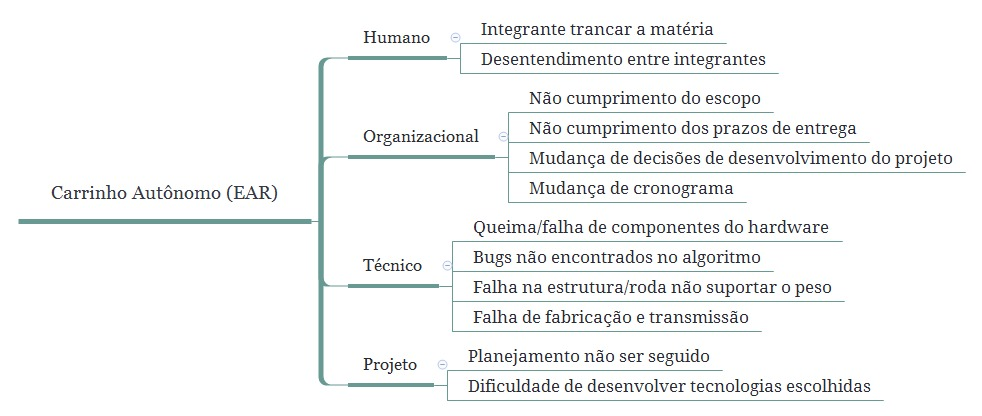
\includegraphics[width=.9\textwidth]{figuras/ear.jpg}
		\caption{Estrutura analítica de Riscos}
		\label{fig:ear}
	\end{figure}

\subsection{Definição de respostas a riscos}

São caracterizadas possíveis medidas para cada risco:

\textbf{Evitar:} 
Modificando o plano de projeto para eliminar a possibilidade, mesmo que não completamente, mas podendo ser evitado.

\textbf{Transferir:} 
Fazer com que sua consequência se torne parte de uma resposta, transferindo-a para outra parte.

\textbf{Mitigar:} 
Reduzir sua consequência, de forma a propor ações preventivas para que sejam mínimas.
 
\par Dessa forma, estratégias são aplicadas aos riscos conforme a define a Tabela \ref{tab:estrategia_riscos}.


% ######## init table ########
\begin{table}[h]
 \centering
% distancia entre a linha e o texto
 {\renewcommand\arraystretch{1.25}
 \caption{Estratégia para riscos} \label{tab:estrategia_riscos}
 \begin{tabular}{ l l }
  \cline{1-1}\cline{2-2}  
    \multicolumn{1}{|c|}{\textbf{Risco} \centering } &
    \multicolumn{1}{c|}{\textbf{Correção} \centering }
  \\  
  \cline{1-1}\cline{2-2}  
    \multicolumn{1}{|p{3.850cm}|}{Integrante trancar a matéria \centering } &
    \multicolumn{1}{p{4.217cm}|}{Transferir \centering }
  \\  
  \cline{1-1}\cline{2-2}  
    \multicolumn{1}{|p{3.850cm}|}{Desentendimento entre integrantes \centering } &
    \multicolumn{1}{p{4.217cm}|}{Mitigar \centering }
  \\  
  \cline{1-1}\cline{2-2}  
    \multicolumn{1}{|p{3.850cm}|}{Não cumprimento do escopo \centering } &
    \multicolumn{1}{p{4.217cm}|}{Evitar \centering }
  \\  
  \cline{1-1}\cline{2-2}  
    \multicolumn{1}{|p{3.850cm}|}{Não cumprimento dos prazos de entrega \centering } &
    \multicolumn{1}{p{4.217cm}|}{Evitar \centering }
  \\  
  \cline{1-1}\cline{2-2}  
    \multicolumn{1}{|p{3.850cm}|}{Mudança de decisões de desenvolvimento do projeto \centering } &
    \multicolumn{1}{p{4.217cm}|}{Evitar \centering }
  \\  
  \cline{1-1}\cline{2-2}  
    \multicolumn{1}{|p{3.850cm}|}{Mudança de cronograma \centering } &
    \multicolumn{1}{p{4.217cm}|}{Mitigar \centering }
  \\  
  \cline{1-1}\cline{2-2}  
    \multicolumn{1}{|p{3.850cm}|}{Queima/falha de componentes do hardware \centering } &
    \multicolumn{1}{p{4.217cm}|}{Mitigar \centering }
  \\  
  \cline{1-1}\cline{2-2}  
    \multicolumn{1}{|p{3.850cm}|}{Bugs não encontrados no algoritmo \centering } &
    \multicolumn{1}{p{4.217cm}|}{Mitigar \centering }
  \\  
  \cline{1-1}\cline{2-2}  
    \multicolumn{1}{|p{3.850cm}|}{Falha na estrutura/roda não suportar o peso \centering } &
    \multicolumn{1}{p{4.217cm}|}{Mitigar \centering }
  \\  
  \cline{1-1}\cline{2-2}  
    \multicolumn{1}{|p{3.850cm}|}{Falha de fabricação e transmissão \centering } &
    \multicolumn{1}{p{4.217cm}|}{Mitigar \centering }
  \\  
  \cline{1-1}\cline{2-2}  
    \multicolumn{1}{|p{3.850cm}|}{Dificuldade de desenvolver tecnologias escolhidas \centering } &
    \multicolumn{1}{p{4.217cm}|}{Mitigar \centering }
  \\  
  \cline{1-1}\cline{2-2}  
    \multicolumn{1}{|p{3.850cm}|}{Planejamento não ser seguido \centering } &
    \multicolumn{1}{p{4.217cm}|}{Evitar \centering }
  \\  
  \hline

 \end{tabular} }
\end{table}





















